\documentclass{csc_assignment4}
\usepackage[utf8]{inputenc}
\usepackage[letterpaper, portrait, margin=1in]{geometry}
\usepackage{calc}  % arithmetic in length parameters
\usepackage{enumitem}  % more control over list formatting
\usepackage{fancyhdr}  % simpler headers and footers
\usepackage{lastpage}  % for last page number
\usepackage{relsize}  % easier font size changes
\usepackage[normalem]{ulem}  % smarter underlining
\usepackage{url}  % verb-like typesetting of URLs
\usepackage{xfrac}  % nicer looking simple fractions for text and math
\usepackage{amsmath}
\usepackage{amssymb}
\usepackage{tikz}
\usepackage{algorithm}
\usepackage{algorithmic}
\usepackage{graphicx}
\usepackage{listings}
\graphicspath{{/}}
\usepackage[export]{adjustbox}
\usepackage{enumitem}
\usepackage{subcaption}

 \lstset{breaklines=true}

% ----------------------------------------------------------------
% TODO: Enter the assignment number, your name, and your student number below
% ----------------------------------------------------------------
\AssignmentName{Assignment 1}
\StudentName{Akhil Gupta}
\StudentNumber{1000357071}

% ----------------------------------------------------------------
\begin{document}
\begin{description}

\item[Q1.]
\begin{enumerate}[label=(\alph*)]
\item
\begin{lstlisting}[language=Python]
import numpy as np
import matplotlib.pyplot as plt
import matplotlib.cm as cm
import scipy.misc as sm

#Read image
img_rgb = sm.imread('image.jpg')
#Allocate space for grayscale version of image
img_gray = np.zeros((img_rgb.shape[0], img_rgb.shape[1]))
#Convert image to grayscale
for row in range(len(img_rgb)):
   for col in range(len(img_rgb[row])):
      img_gray[row][col] = np.average(img_rgb[row][col])

#Setup variables to store filter h&w and image h&w
img_filter = np.array([[-1,-1,-1],[-1,4,-1],[-1,-1,-1]])
img_height = img_gray.shape[0]
img_width = img_gray.shape[1]
filter_height = img_filter.shape[0]
filter_width = img_filter.shape[1]

#Function to perform 2D correlation with image and filter
def correlate(padded_img, filter):
   img_output = np.zeros((img_height, img_width))
   for i in range(img_width):
      for j in range(img_height):
         img_output[j][i] = (filter*padded_img[j:j+filter_height, i:i+filter_width]).sum()

   return img_output

#Add "zero-pad" to deal with border of the image
padded_img = np.zeros((img_height + 2, img_width + 2))   
padded_img[1:-1, 1:-1] = img_gray
output = correlate(padded_img, img_filter)

#Plots
fig1 = plt.figure()
plt.imshow(img_gray, cmap=cm.Greys_r)
fig1.suptitle("Original Grayscale Image")

fig2 = plt.figure()
plt.imshow(output, cmap=cm.Greys_r)
fig2.suptitle("Correlated Grayscale Image")

plt.show()
\end{lstlisting}

\item   
\begin{lstlisting}[language=Python]
#Same import statements
#Read image (from (a))

#Setup variables to store filter h&w and image h&w
img_filter = np.array([[-1,-1,-1],[-1,4,-1],[-1,-1,-1]])[..., None]
img_filter_3d = np.repeat(img_filter, 3, axis=2)
img_height = img_gray.shape[0]
img_width = img_gray.shape[1]
img_depth = img_rgb.shape[2]
filter_height = img_filter.shape[0]
filter_width = img_filter.shape[1]

#Function to perform 2D correlation with image and filter (from (a))

#Function to perform 2D correlation with rgb image and 3D filter
def correlate_3d(padded_img, filter):
	img_output = np.zeros((img_height, img_width))
	for i in range(img_width):
		for j in range(img_height):
			img_output[j][i] = (filter*padded_img[j:j+filter_height, i:i+filter_width, :]).sum()

	return img_output

#Calculate number of padding zeros to add
padding_height = ((img_height - 1) + (filter_height - img_height)) 
padding_width = ((img_width - 1) + (filter_width - img_width))
padding_top = padding_height // 2
padding_bottom = padding_height - padding_top
padding_left = padding_width // 2
padding_right = padding_width - padding_left

#Add "zero-pad" to deal with top, bottom, left and right of image
padded_rgb_img = np.zeros((img_height + padding_height, img_width + padding_width, img_depth))
padded_rgb_img[padding_top:-padding_bottom, padding_left:-padding_right, :] = img_rgb
output_rgb = correlate_3d(padded_rgb_img, img_filter_3d)

#Plots
fig3 = plt.figure()
plt.suptitle("Original RGB Image")
plt.imshow(img_rgb)

fig4 = plt.figure()
plt.suptitle("Correlated RGB Image")
plt.imshow(output_rgb)

plt.show()
\end{lstlisting}
\end{enumerate}

\item[Q2.]
\begin{enumerate}[label=(\alph*)]
\item We have a $n$ x $n$ image which means $n^{2}$ pixels. We perform $m^{2}$ operations per pixel, hence, total computational cost of computing convolution is $O(n^{2}m^{2})$. The computational cost if $h$ is a separable filter gives us $2m$ operations per pixel, hence, total computational cost is $O(2mn^{2})$ = $O(mn^{2})$.

\item
\begin{lstlisting}[language=Python]
def create_gauss_filter(sigma_x, sigma_y):
	sigma = math.sqrt((sigma_x)**2 + (sigma_y)**2)
	# creates filter of shape based on mathworks imgaussfilt fn
	shape = 2 * math.ceil(2*sigma)+1
	u, v = np.mgrid[-shape:shape+1, -shape:shape+1]
	const = 2 * (sigma**2)
	h = np.exp(-((u**2 + v**2)/const))
	return h/(math.pi*const)
\end{lstlisting}

\item
\begin{lstlisting}[language=MATLAB]
% read image
im = imread('image.jpg');
% convert to grayscale
img = rgb2gray(im);

% instead of applying two filters, we can apply one 
% by sqrt(sigma_x^2 + sigma_y^2)
sigma = sqrt(1.^2 + 10.^2);
% applies 10x10 filter
h = fspecial('gaussian', [10,10], sigma);
out = imfilter(img, h, 'conv');
imshow(out);
\end{lstlisting}
\newpage
\begin{figure}[h]
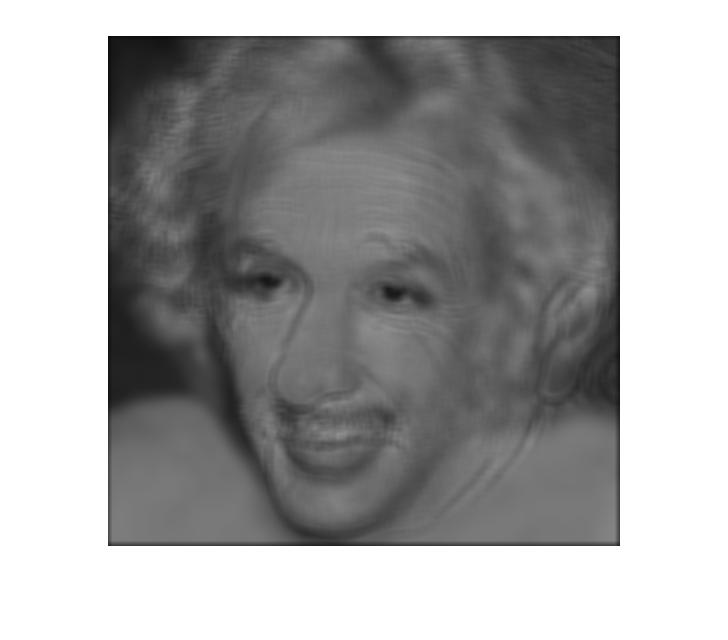
\includegraphics[width=0.6\textwidth, center]{q2c.jpg}
\vspace*{-20mm}
\caption{Convolved image with 2D Gaussian filter with $\sigma_{x} = 1$ and $\sigma_{y} = 10$}
\end{figure}

\item We know that Gaussian filters are separable, i.e. they can be written as a product of 2 1D-filters. Hence, even the partial derivatives of a Gaussian filter are separable. So, yes, the horizontal derivative, $\cfrac{\partial G(x,y)}{\partial x}$, of a Gaussian filter G is separable. \\ $G(x, y) = \cfrac{1}{2\pi\sigma^{2}}e^{\cfrac{-(x^{2}+y^{2})}{\sigma^{2}}} = 
(\cfrac{1}{\sqrt{2\pi}\sigma}e^{\cfrac{-x^{2}}{\sigma^{2}}}) * (\cfrac{1}{\sqrt{2\pi}\sigma}e^{\cfrac{-y^{2}}{\sigma^{2}}}) = g_{x} * g_{y}$\\
$\cfrac{\partial G(x,y)}{\partial x} = \cfrac{\partial ({\cfrac{1}{\sqrt{2\pi}\sigma}e^{\cfrac{-x^{2}}{\sigma^{2}}}) * (\cfrac{1}{\sqrt{2\pi}\sigma}e^{\cfrac{-y^{2}}{\sigma^{2}}})}}{\partial x}$ \\
$ = \cfrac{\partial ({\cfrac{1}{\sqrt{2\pi}\sigma}e^{\cfrac{-x^{2}}{\sigma^{2}}})}}{\partial x} * ({\cfrac{1}{\sqrt{2\pi}\sigma}e^{\cfrac{-y^{2}}{\sigma^{2}}})} + \cfrac{\partial ({\cfrac{1}{\sqrt{2\pi}\sigma}e^{\cfrac{-y^{2}}{\sigma^{2}}})}}{\partial x} * ({\cfrac{1}{\sqrt{2\pi}\sigma}e^{\cfrac{-x^{2}}{\sigma^{2}}})}$ \\ $ = \cfrac{\partial ({\cfrac{1}{\sqrt{2\pi}\sigma}e^{\cfrac{-x^{2}}{\sigma^{2}}})}}{\partial x} * ({\cfrac{1}{\sqrt{2\pi}\sigma}e^{\cfrac{-y^{2}}{\sigma^{2}}})} + 0$ \\ $ = \cfrac{-x}{\sigma^{2}} * ({\cfrac{1}{\sqrt{2\pi}\sigma}e^{\cfrac{-y^{2}}{\sigma^{2}}})} = \cfrac{-x}{\sigma^{2}} * g_{y}$ = product of 2 1D-filters.

\vspace{4mm}
\item Given a filter F, we can check whether it's separable or not by looking at the rank of the filter matrix. If the rank $= 1$, i.e. all rows of the matrix are scalar multiples of each other.
\newpage
\end{enumerate}

\item[Q3.]
\begin{enumerate}[label=(\alph*)]
\item
\begin{lstlisting}[language=MATLAB]
% read image & convert to grayscale
im = imread('waldo.png');
template = imread('template.png');
img = rgb2gray(im);
template = rgb2gray(temp);

output_img = q3a(img);
output_template = q3a(template);

function out = q3a(image)
% calculate magnitude of gradient
[Gx, Gy] = imgradientxy(image);
Gmag = sqrt(Gx.^2 + Gy.^2);
imshow(Gmag, []);
out = Gmag;
end
\end{lstlisting}

\begin{figure}[h]
\centering
\begin{subfigure}{0.5\textwidth}
\centering
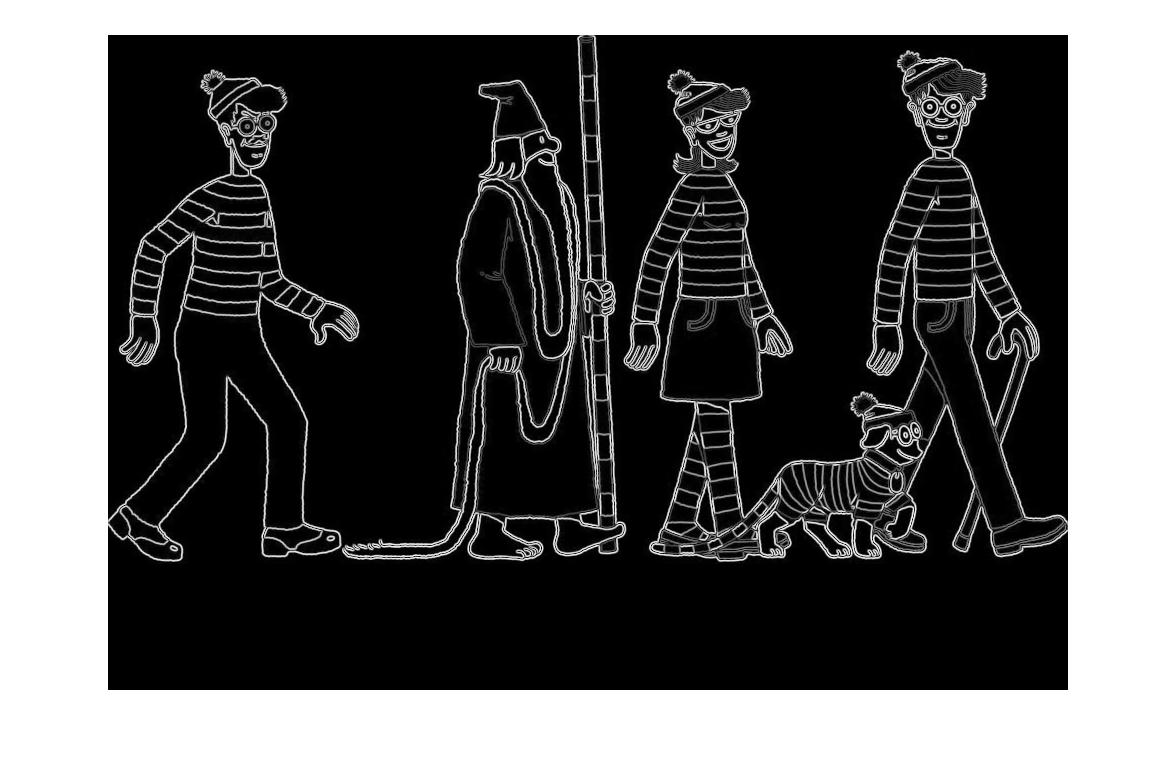
\includegraphics[width=1.2\linewidth, height=7cm]{q3a1.jpg}
\vspace{-10mm}
\caption{Magnitude of gradient for waldo.png}
\end{subfigure}
\begin{subfigure}{0.5\textwidth}
\centering
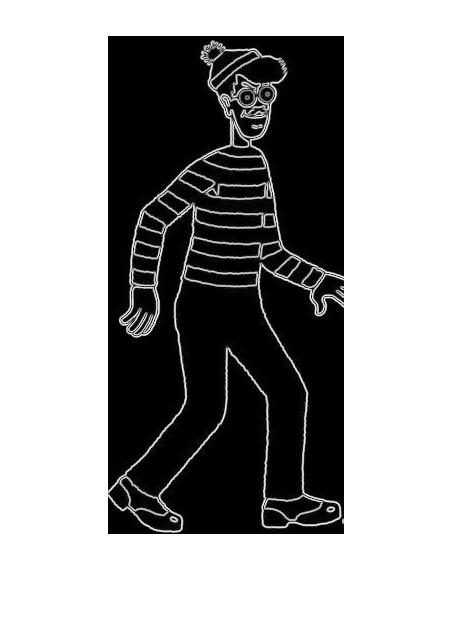
\includegraphics[width=0.5\linewidth, height=6cm]{q3a2.jpg}
\vspace{-5mm}
\caption{Magnitude of gradient for template.png}
\end{subfigure}
\end{figure}

\newpage
\item 
\begin{lstlisting}[language=MATLAB]
% read image and template from q3a)
output = q3b(im, template);

function out = q3b(im, template)
% convert image (and template) to grayscale
im_input = im;
im = rgb2gray(im);
im = double(im);
template = rgb2gray(template);
template = double(template);
template = template/sqrt(sum(sum(template.^2)));

% get magnitude of gradients from q3a)
G_im = q3a(im);
G_temp = q3a(template);

% normalized cross-correlation
out = normxcorr2(G_temp, G_im);

% plot the cross-correlation results
figure('position', [100,100,size(out,2),size(out,1)]);
subplot('position',[0,0,1,1]);
imagesc(out)
axis off;
axis equal;

% find the peak in response
[y,x] = find(out == max(out(:)));
y = y(1) - size(template, 1) + 1;
x = x(1) - size(template, 2) + 1;

% plot the detection's bounding box
figure('position', [300,100,size(im,2),size(im,1)]);
subplot('position',[0,0,1,1]);
imshow(im_input);
axis off;
axis equal;
rectangle('position', [x,y,size(template,2),size(template,1)], 'edgecolor', [0.1,0.2,1], 'linewidth', 3.5);

end
\end{lstlisting}

\begin{figure}[h]
\centering
\begin{subfigure}{0.5\textwidth}
\centering
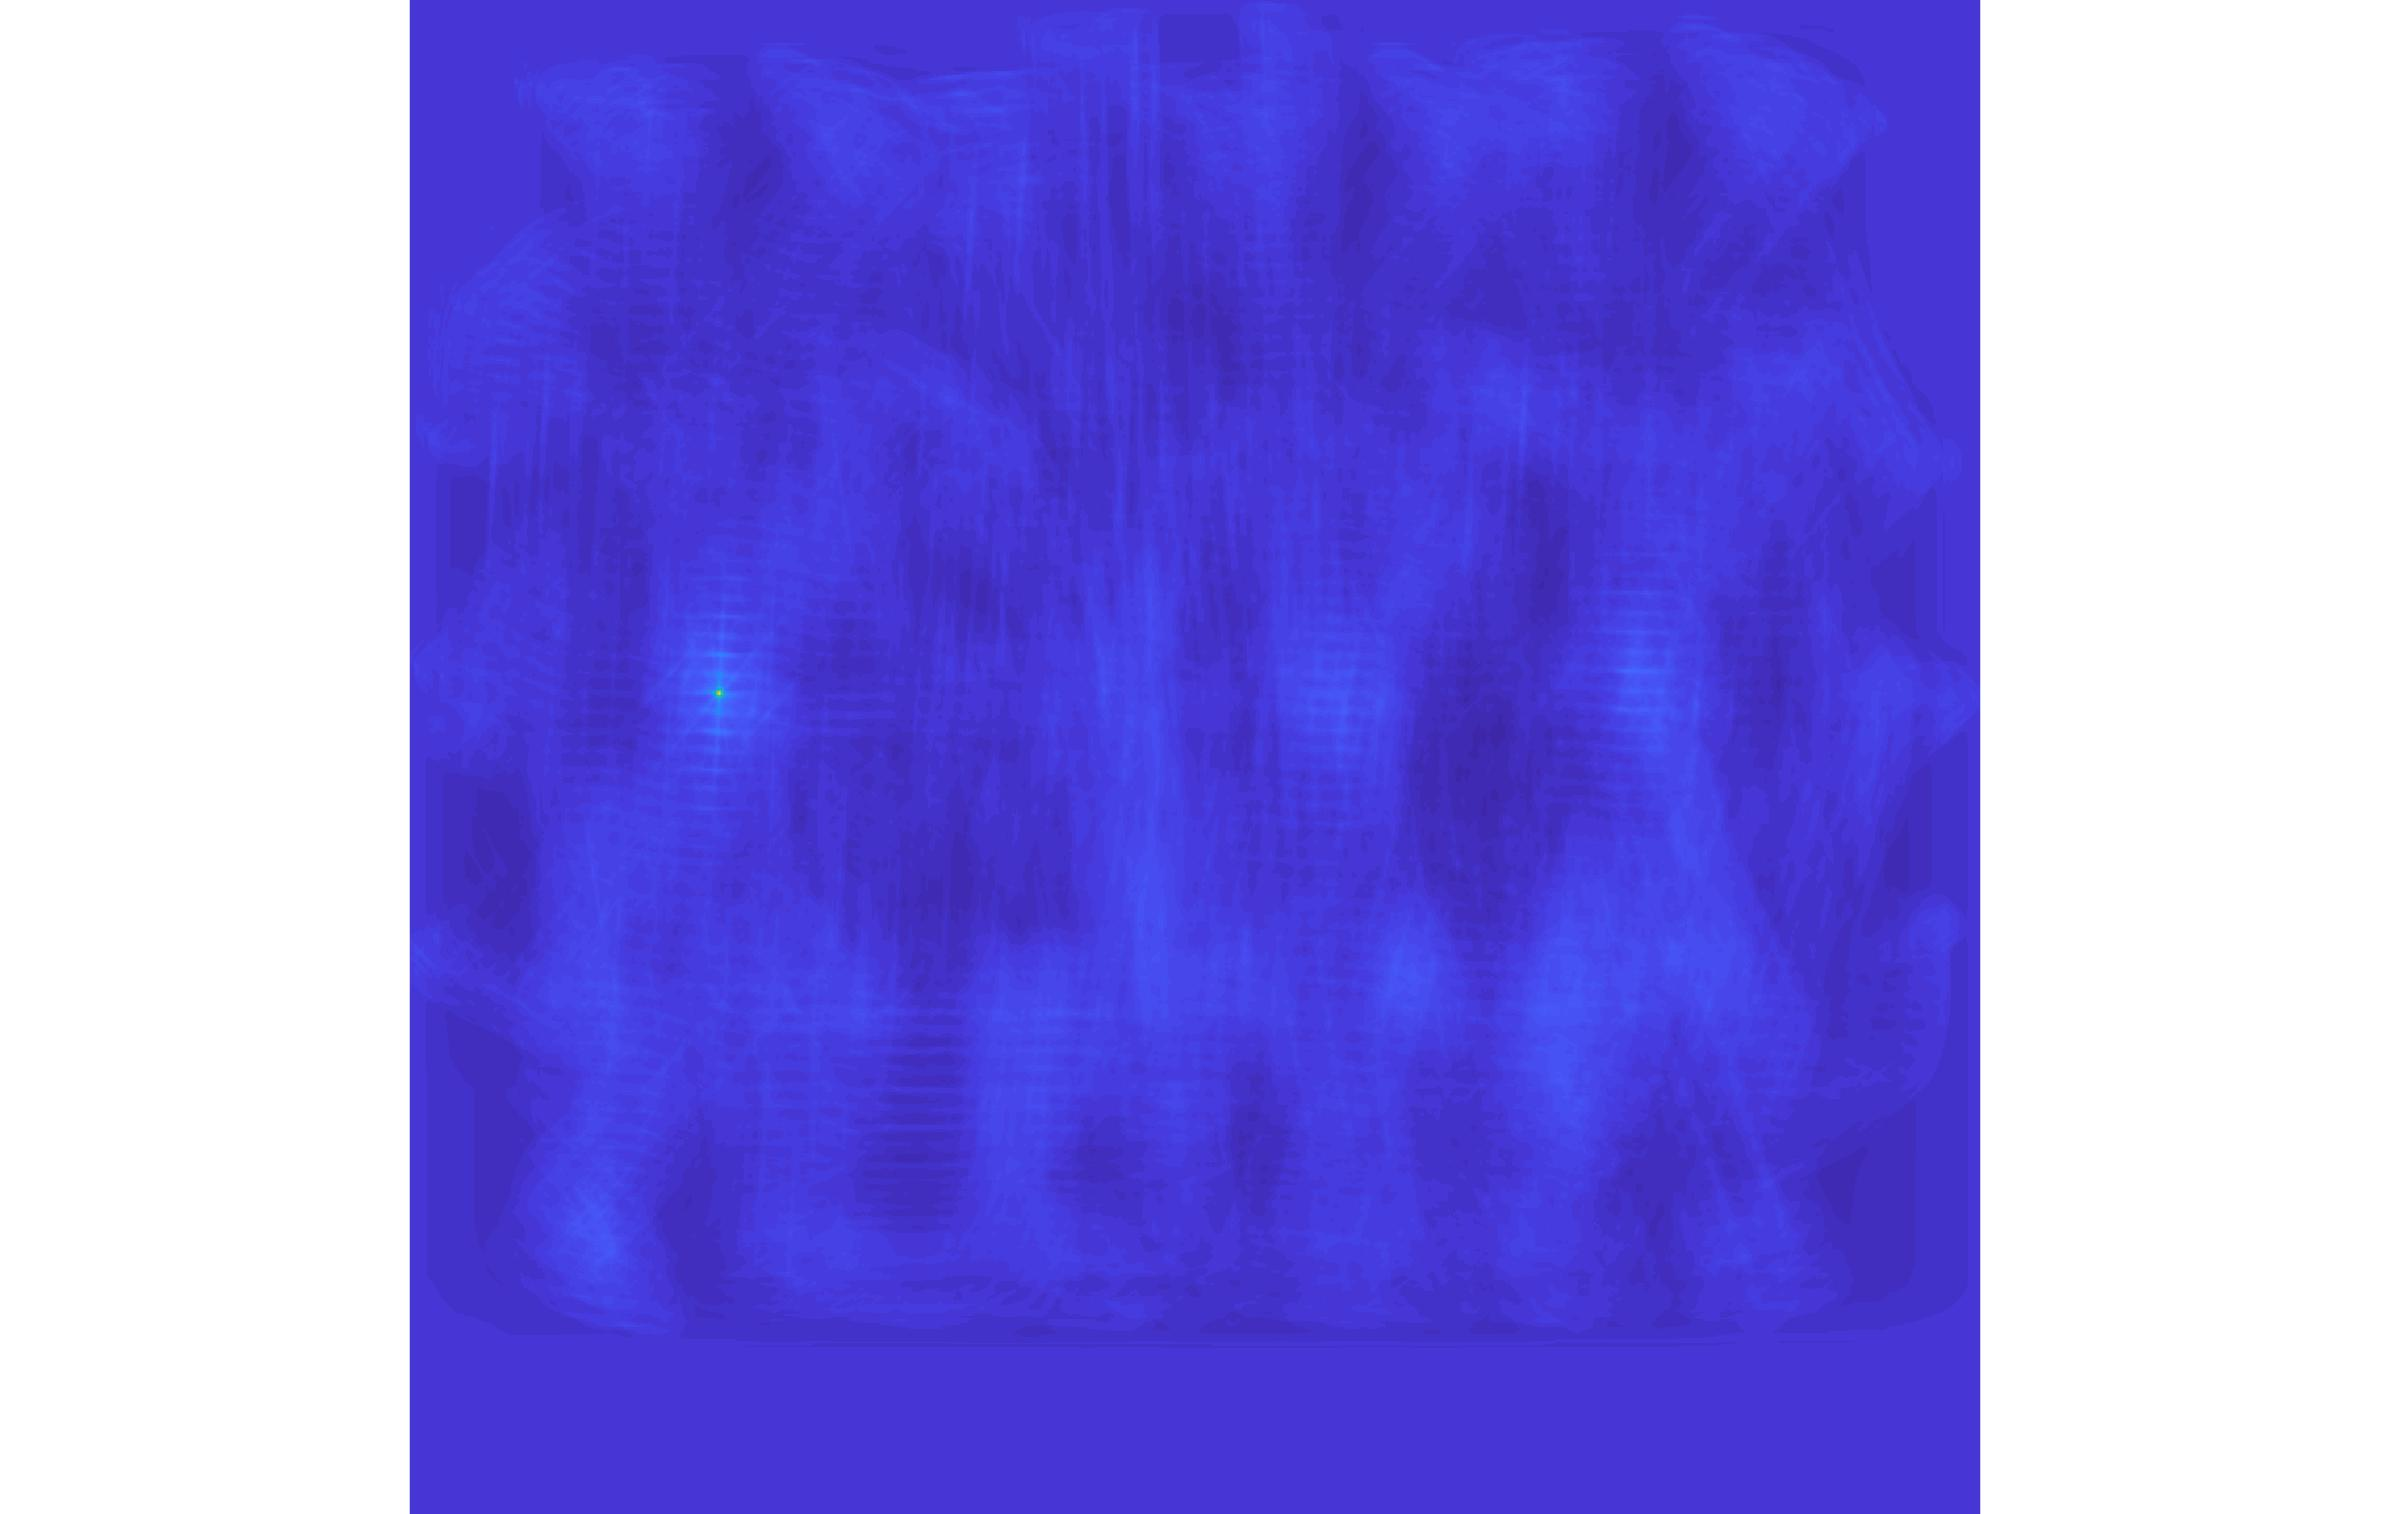
\includegraphics[width=1.2\linewidth, height=7cm]{q3b1.jpg}
\vspace{-2mm}
\caption{Normalized cross-correlation of waldo.png}
\end{subfigure}
\begin{subfigure}{0.5\textwidth}
\centering
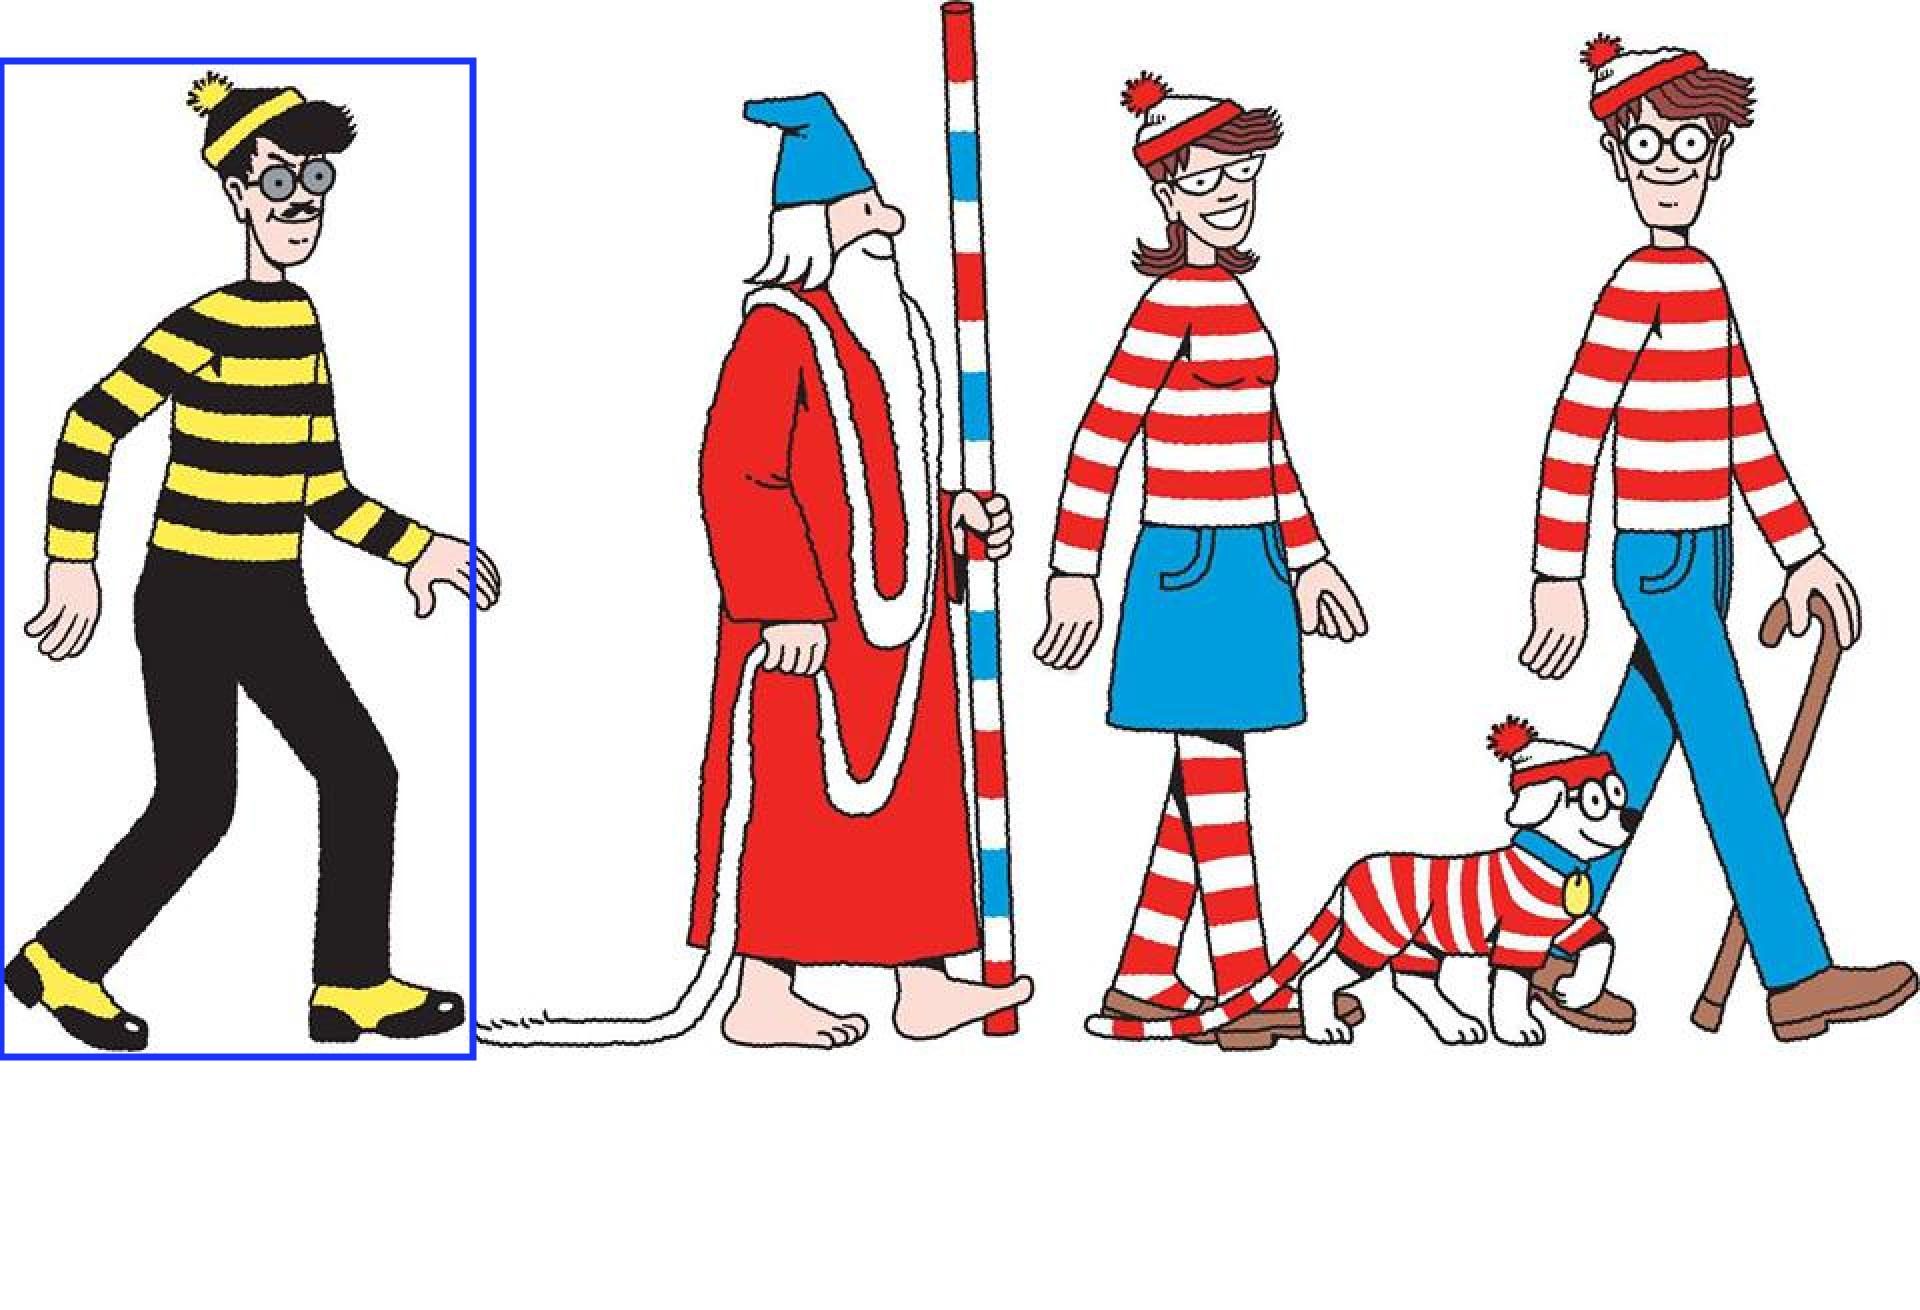
\includegraphics[width=1.2\linewidth, height=6cm]{q3b2.jpg}
\vspace{-15mm}
\caption{Waldo detection localized by template.png}
\end{subfigure}
\begin{subfigure}{0.5\textwidth}
\centering
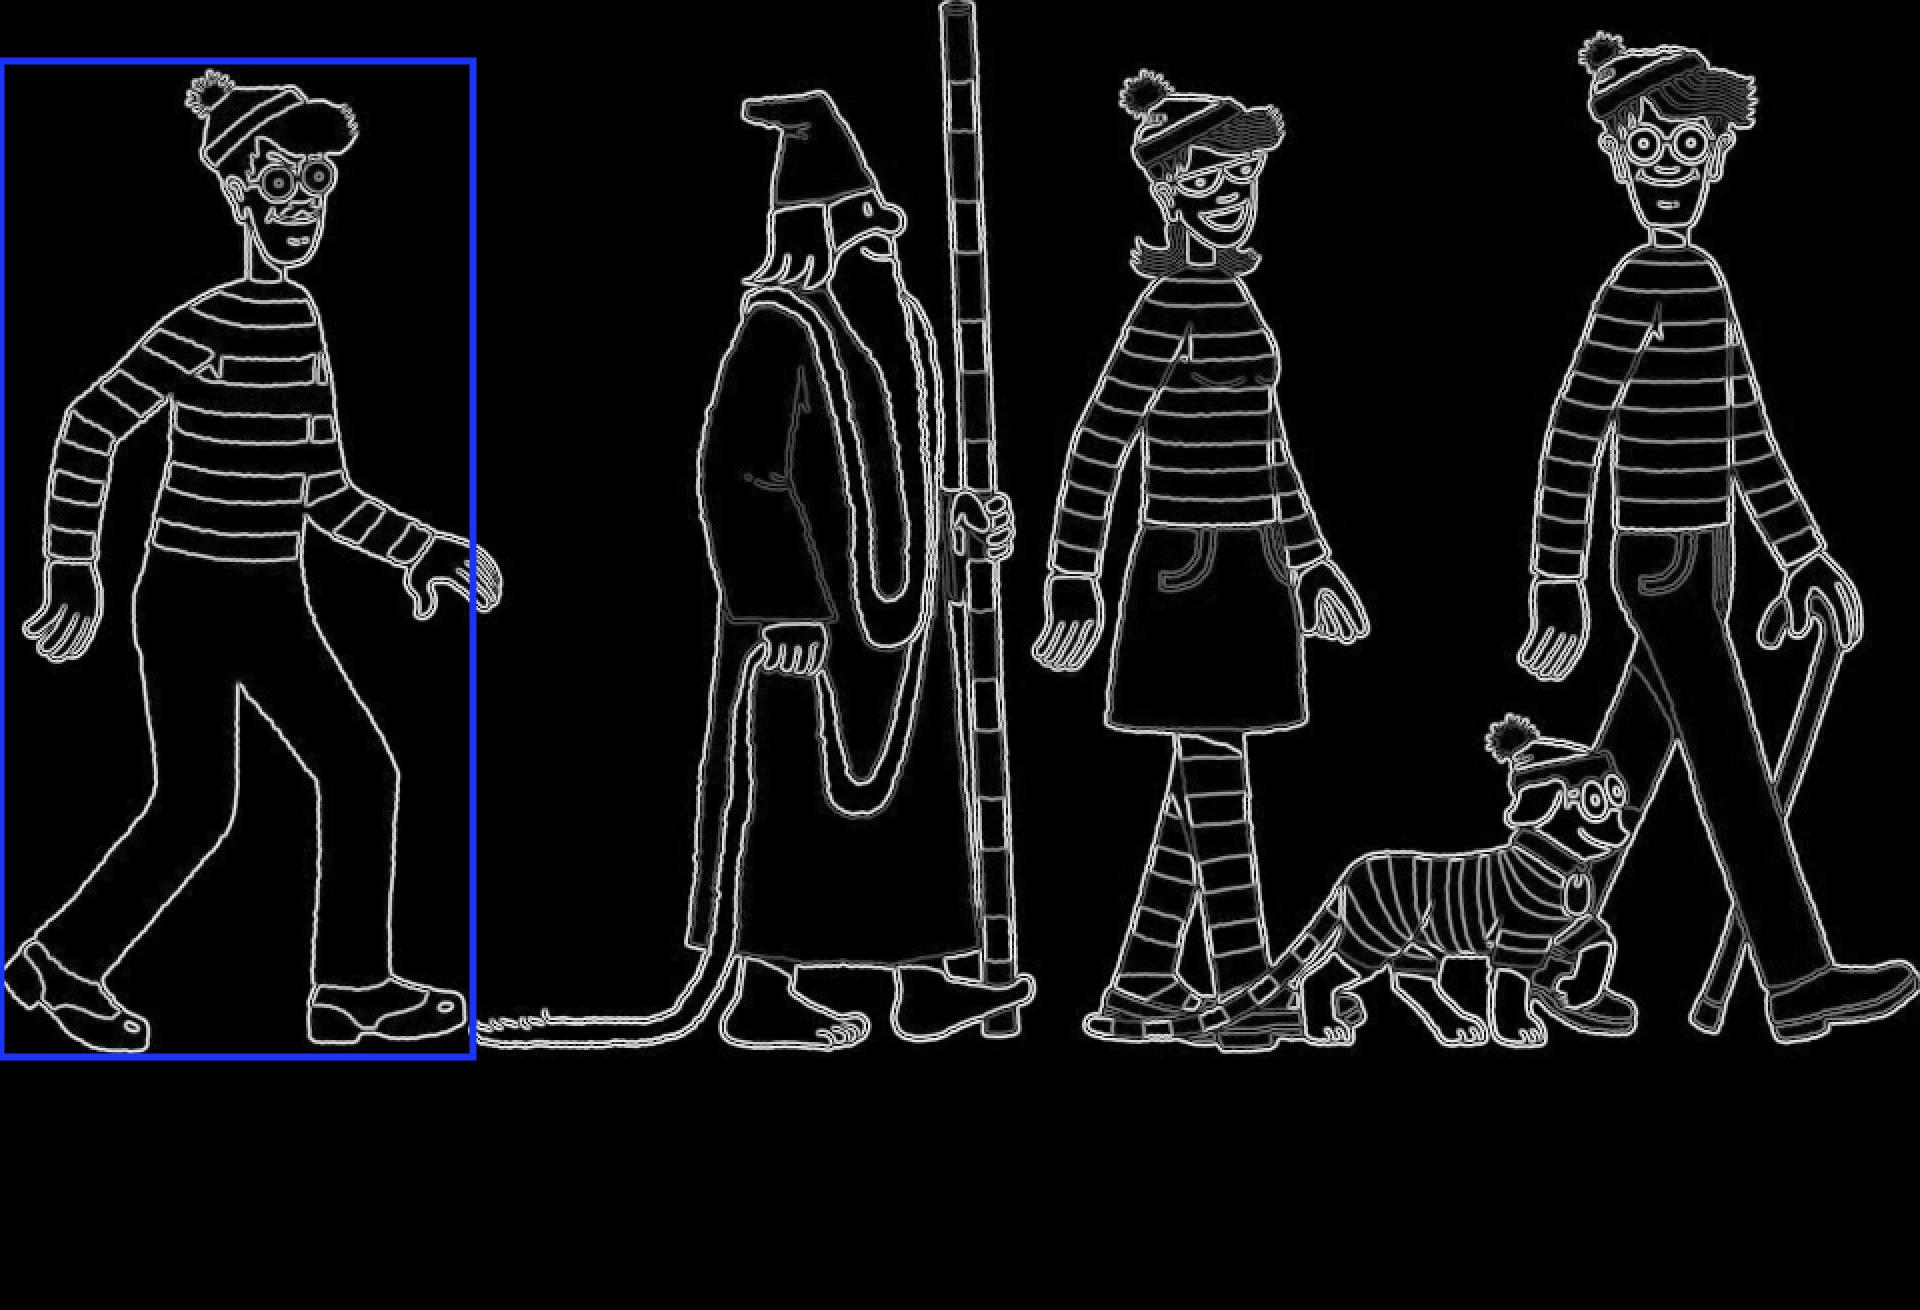
\includegraphics[width=1.2\linewidth, height=6cm]{q3b3.jpg}
\vspace{-5mm}
\caption{Waldo detection (gradient) localized by template.png}
\end{subfigure}
\end{figure}
\clearpage


\item[Q4.]
\begin{enumerate}[label=(\alph*)]
\item Canny edge detector performs the following steps: \\
\begin{itemize}
\item Filter image with derivative of Gaussian (horizontal and vertical):\\
The first step is to apply a smoothing via Gaussian blur to filter out any noise from the image. Then, we calculate the horizontal and vertical derivatives at every point in the image. Larger values of $\sigma$ helps us detect edges of larger scale, whereas smaller values of $\sigma$ helps us detect finer structures. The horizontal derivative tells us the places where there is a rapid change in intensity along the x-axis, whereas the vertical derivative tells us along the y-axis. We use the Sobel Kernel to do so. 
\item Find magnitude and orientation of gradient: \\
The horizontal and vertical derivatives of the image together make up the gradient of the image. The magnitude of the gradient is simply the square root of the sum of squares of the horizontal and vertical derivatives. The magnitude at a particular point tells us whether there lies an edge or not. A high gradient magnitude tells us that there is a drastic change in the intensity of the colours - implying an edge. Also, the direction of the gradient shows which way the edge is oriented.
\item Non-maxima supression: \\
This is a crucial step that separates canny from other edge detectors. As the name of the step implies, it iterates over all the pixels and supresses the ones that are not a local maxima along the gradient direction. This leads to thinning and sharp edges as neighbouring pixels of lower intesity are supressed and only the local maxima survives. As a result, we may lose some edges thus creating gaps in the overall edges. This is fixed in the next step. 
\item Linking and thresholding (hysteresis): \begin{itemize}
\item Define two thresholds: low and high
\item Use the high threshold to start edge curves and the low threshold to continue them \\
In the previous step, we got some very good and thin edges but we lost some edges as well. To fix this, we use a high threshold (strong edges) to start the lost edge curves and a low threshold (weak edges) to continue them based on the direction of the gradient. A combination of this high threshold and low threshold is called hysteresis threshold and we perform this by iterating over all the pixels in the image until the image stops changing. 
\end{itemize}
\end{itemize}
\newpage
\item 
\begin{lstlisting}[language=MATLAB]
im = imread('court.jpg');
img = rgb2gray(im);
canny = edge(img, 'canny', [0, 0.50]);
imshow(canny);
\end{lstlisting}
\begin{figure}[h]
\centering
\begin{subfigure}{0.5\textwidth}
\centering
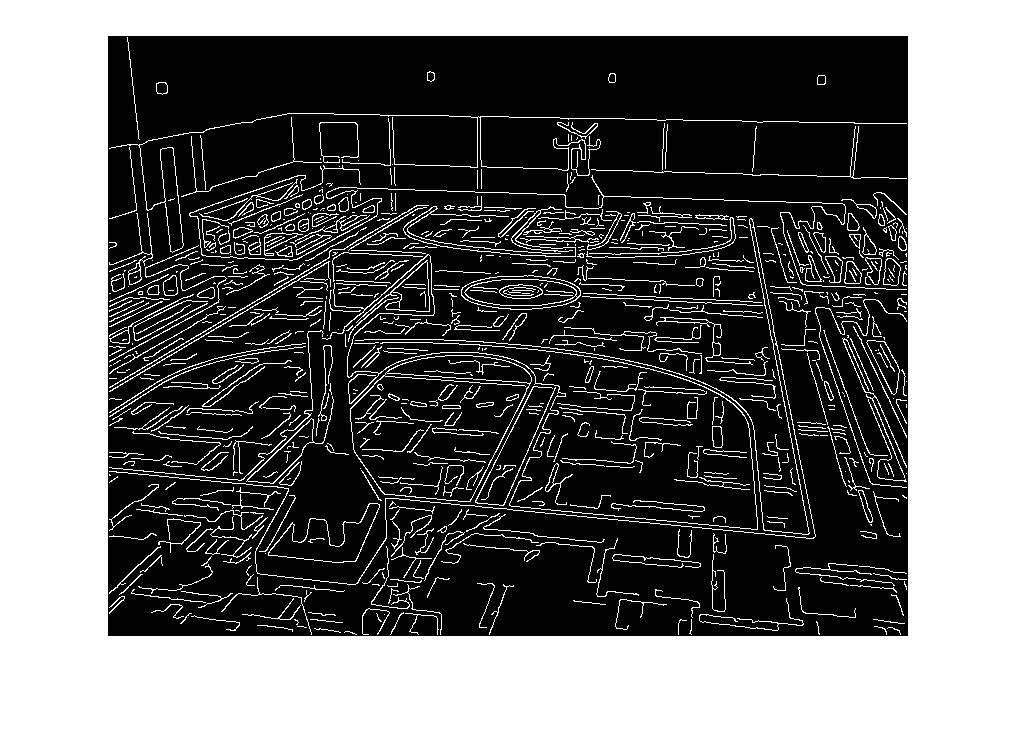
\includegraphics[width=1.2\linewidth, height=7cm]{q4b2.jpg}
\vspace{-10mm}
\caption{Canny edge detector on court.jpg before threshold}
\end{subfigure}
\begin{subfigure}{0.5\textwidth}
\centering
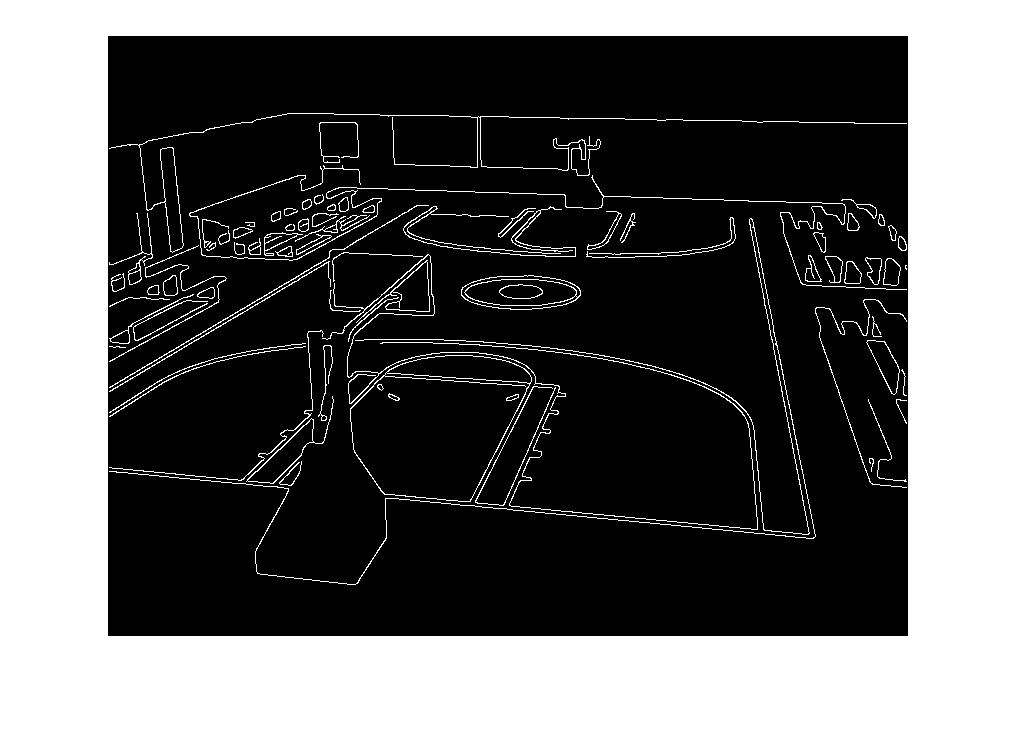
\includegraphics[width=1.2\linewidth, height=7cm]{q4b.jpg}
\vspace{-10mm}
\caption{Canny edge detector on court.jpg after threshold}
\end{subfigure}
\end{figure}
\end{enumerate}
\end{enumerate}

\newpage
\item[Q5.]
\begin{lstlisting}[language=MATLAB]
function out = seam_carving(image)

% read image and convert to grayscale
im = imread(image);
[rows, cols, dim] = size(im);
img = rgb2gray(im);

% compute gradients
[Gx, Gy] = imgradientxy(img);
Gmag = sqrt(Gx.^2 + Gy.^2);
[row_g, col_g, ~] = size(Gmag);
seam_img(1,:) = Gmag(1,:);
seam_img = zeros(row_g, col_g);

% calculate horizontal seam
for col = 2:rows
    for row = 1:rows
        if (row == 1)
            min_energy = min([seam_img(row, col - 1), seam_img(row + 1, col-1)]);
        elseif (row == rows)
            min_energy = min([seam_img(row - 1, col - 1), seam_img(row, col - 1)]);
        else
            min_energy = min([seam_img(row - 1, col - 1), seam_img(row,col - 1), seam_img(row + 1, col - 1)]);
        end
        seam_img(row, col) = Gmag(row, col) + min_energy;
    end
end

seam_img = Gmag;

% calculate min value 
[val, index] = min(seam_img(:, cols));
seam = zeros(cols, 1);
seam(cols) = index;

while cols > 1
    cols = cols - 1;
    min_val = seam_img(index, cols);
    i = index;
    
    if index ~= 1
        if seam_img(index - 1, cols) < min_val
            min_val = seam_img(index - 1, cols);
            i = index - 1;
        end
    end

    if index ~= cols
        if seam_img(index + 1, cols) < min_val
            i = index + 1;
        end 
    end
    
    seam(cols) = i;
    index = i;
end

% remove seam
for dim = 1:3
    for col = 1:cols
        for row = seam(col):rows - 1
            im(row, col, dim) = im(row + 1, col, dim);
        end
    end
end
removed_output = im(1:rows - 1, :, :);

im = removed_output;

% show seam
for i = 1:size(seam, 1)
    im(seam(i), i, 1:3) = 0;
end

imshow(im);

*** OUTPUT ON NEXT PAGE ***
\end{lstlisting}
\clearpage
\begin{figure}[h]
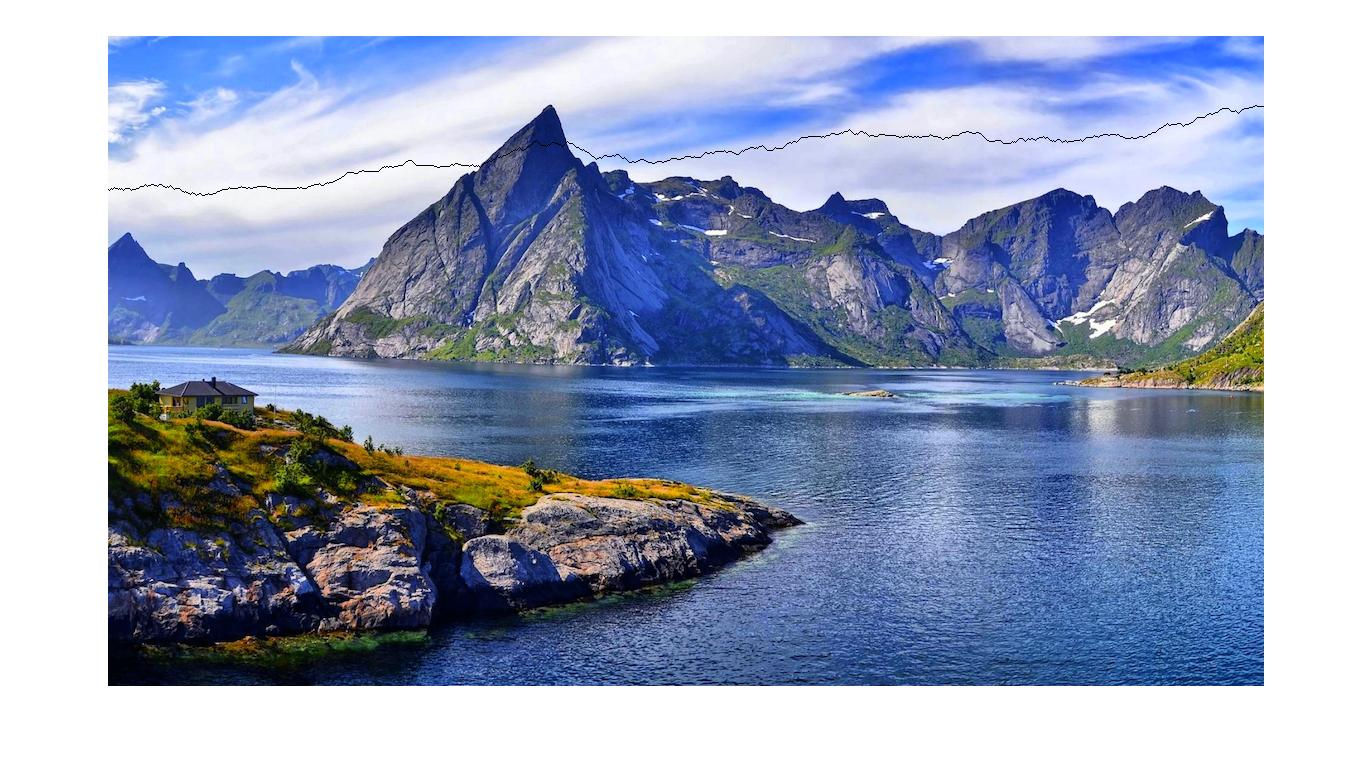
\includegraphics[width=1.0\textwidth, center]{seam.jpg}
\vspace*{-15mm}
\caption{Output of seam-carving algorithm to find skyline (shown in black)}
\end{figure}


\end{description}
\end{document}
  
  



